% ============================================================================
% Việc 5.05 - Đối chiếu thực nghiệm với lý thuyết
% Số liệu: results/time_mem.csv (bậc hai), results/time_mem_cubic.csv (bậc ba) của việc 5.02
% Tái tạo bảng và hình: python3 scripts/analyze_complexity.py
% Cần trong preamble: \usepackage{graphicx}. Hình: figures/loglog_time_vs_n.pdf
% ============================================================================

\subsection{Đối chiếu thực nghiệm với lý thuyết}
\label{sec:kiemchung}

Mục này kiểm tra thời gian chạy đo được có tăng theo $N$ đúng bậc đã chứng minh ở các mục trước hay không.
Nếu $T(N) \approx C \cdot N^{b}$ thì $\log T = b \log N + \log C$, nên trên đồ thị log-log thời gian là
một đường thẳng có độ dốc bằng số mũ $b$, còn hằng số $C$ chỉ tịnh tiến đường thẳng.
Vì vậy độ dốc cho phép so sánh bậc tăng trưởng mà không phụ thuộc máy chạy.

\subsubsection{Dữ liệu và cách ước lượng}
Dữ liệu lấy từ benchmark ở mục~\ref{sec:thucnghiem}: 20 tổ hợp tham số
($M \in \{4, 8, 16, 32\}$; $(\alpha, \beta) \in \{(1{,}2; 1), (1{,}2; 10), (4; 1), (4; 10), (4; 100)\}$),
mỗi tổ hợp 5 seed, với $N \in \{10^3, 10^4, 10^5\}$, cho cả mô hình năng lượng bậc hai và bậc ba.
Thời gian dùng là \texttt{time\_ms} do solver tự đo bằng \texttt{std::chrono}, chỉ gồm phần giải,
không gồm khởi động tiến trình và đọc JSON.
Với mỗi cấu hình (mô hình, solver, $M$, $\alpha$, $\beta$, seed) chúng tôi hồi quy bình phương tối thiểu
$\log_{10} T$ theo $\log_{10} N$, thu được 100 giá trị độ dốc cho mỗi cặp (mô hình, solver),
rồi báo cáo trung bình $\bar b$, độ lệch chuẩn $s$ và khoảng tin cậy 95\% của trung bình theo phân phối Student.

Hai nhóm dòng bị loại khỏi hồi quy.
Thứ nhất, DP gốc với $N = 10^5$ cần $M N^2 \ge 10^{10}$ phép tính nên bị ngắt;
giá trị trong file kết quả là ngoại suy bằng 100 lần thời gian ở $N = 10^4$,
tức đã giả định sẵn độ dốc bằng 2, nên đưa vào hồi quy sẽ là lập luận vòng.
Độ dốc của DP gốc vì vậy chỉ ước lượng từ hai điểm $N = 10^3$ và $10^4$.
Thứ hai, CHT không chạy với mô hình bậc ba, vì $(S_i - S_k)^3$ có các số hạng trộn
$S_i^2 S_k$ và $S_i S_k^2$ nên không đưa được về dạng đường thẳng (mục~\ref{sec:cht}).

Giá trị lý thuyết của độ dốc cần được tính cẩn thận.
Hàm $N \log N$ không phải đường thẳng trên đồ thị log-log;
độ dốc cát tuyến của nó trên đoạn $[10^3, 10^5]$ là
\[
  \frac{1}{2}\log_{10}\frac{10^5 \ln 10^5}{10^3 \ln 10^3} \approx 1{,}111,
\]
(1{,}125 trên $[10^3, 10^4]$ và 1{,}097 trên $[10^4, 10^5]$).
Vì vậy một thuật toán $O(MN\log N)$ được kỳ vọng có độ dốc khoảng 1{,}11 trên dải $N$ này, chứ không phải đúng 1.

\begin{table}[t]
  \centering
  \caption{Độ dốc log-log của thời gian giải theo $N$. Mỗi dòng 100 cấu hình, trừ CHT tách theo nhánh cài đặt (deque: 15, cây phân đoạn: 85).}
  \label{tab:dodoc}
  \footnotesize
  \setlength{\tabcolsep}{2.5pt}
  \begin{tabular}{llccc}
    \hline
    Mô hình & Solver & Lý thuyết & $\bar b \pm s$ & KTC 95\% \\
    \hline
    Bậc hai & DP gốc            & 2      & $2{,}022 \pm 0{,}087$ & $[2{,}005; 2{,}039]$ \\
            & D\&C              & 1{,}111 & $1{,}092 \pm 0{,}039$ & $[1{,}084; 1{,}100]$ \\
            & CHT deque & 1      & $0{,}996 \pm 0{,}043$ & $[0{,}972; 1{,}019]$ \\
            & CHT cây PĐ & 1{,}111 & $1{,}113 \pm 0{,}030$ & $[1{,}106; 1{,}119]$ \\
    \hline
    Bậc ba  & DP gốc            & 2      & $2{,}074 \pm 0{,}120$ & $[2{,}050; 2{,}098]$ \\
            & D\&C              & 1{,}111 & $1{,}078 \pm 0{,}045$ & $[1{,}069; 1{,}087]$ \\
    \hline
  \end{tabular}
\end{table}

\begin{figure*}[t]
  \centering
  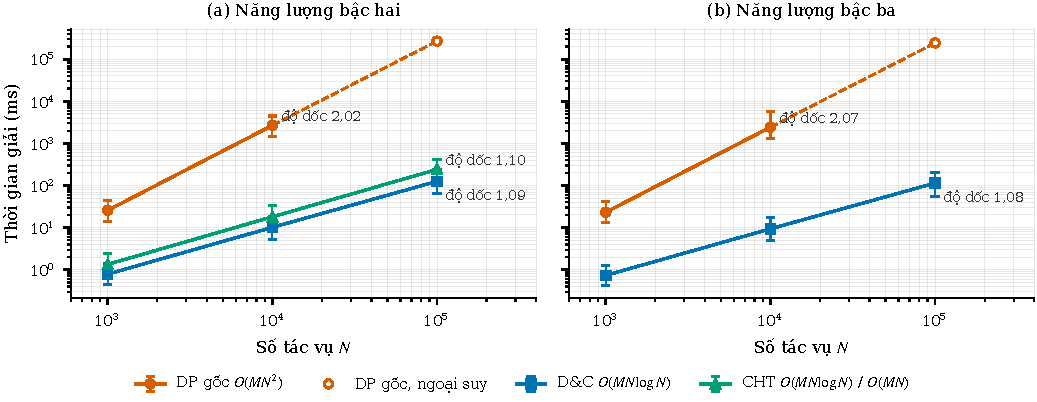
\includegraphics[width=\textwidth]{figures/loglog_time_vs_n.pdf}
  \caption{Thời gian giải theo $N$ trên thang log-log. Điểm là trung vị của 100 cấu hình,
  thanh lỗi là khoảng tứ phân vị. Điểm rỗng của DP gốc tại $N = 10^5$ là ngoại suy, không dùng để tính độ dốc.
  Số ghi cạnh mỗi đường là độ dốc trung bình ở Bảng~\ref{tab:dodoc}.}
  \label{fig:loglog}
\end{figure*}

\subsubsection{Kết quả}
Bảng~\ref{tab:dodoc} và Hình~\ref{fig:loglog} cho thấy ba nhóm tách biệt rõ:
DP gốc có độ dốc khoảng 2, còn D\&C và CHT có độ dốc khoảng 1{,}1,
khớp với bậc $O(MN^2)$ và $O(MN\log N)$ đã chứng minh.
Tính theo trung vị, D\&C nhanh hơn DP gốc khoảng 33 lần ở $N = 10^3$ và 264 lần ở $N = 10^4$ (bậc hai;
bậc ba: 31 và 259 lần). Khi $N$ tăng 10 lần, tỷ số này tăng khoảng 8 lần, gần với mức 7{,}5 lần mà tỷ số
$N / \log N$ dự đoán.

\paragraph{DP gốc}
Độ dốc 2{,}02 (bậc hai) và 2{,}07 (bậc ba) cao hơn 2 một chút.
Chi phí trung bình trên mỗi phép toán, tính bằng $T / (MN^2/2)$, tăng từ 4{,}4 lên 5{,}1~ns (bậc hai)
và từ 4{,}2 lên 6{,}1~ns (bậc ba) khi $N$ tăng từ $10^3$ lên $10^4$.
Một giải thích hợp lý là ở $N = 10^3$ các mảng \texttt{prev}, $S$, $d$ chỉ vài chục KB và nằm gọn trong cache L1,
còn ở $N = 10^4$ thì không; giả thuyết này chưa được kiểm chứng bằng profiler.
Độ lệch lớn nhất ở bậc ba với $M = 32$ (2{,}22).
Vì chỉ có hai điểm đo, độ dốc của DP gốc cũng có độ phân tán lớn nhất ($s = 0{,}09$ đến $0{,}12$).

\paragraph{D\&C Optimization}
Độ dốc 1{,}09 (bậc hai) và 1{,}08 (bậc ba) nằm giữa 1 và giá trị cát tuyến 1{,}111;
khoảng tin cậy loại trừ cả 1 lẫn 1{,}111, tức thời gian tăng nhanh hơn tuyến tính nhưng chậm hơn $N\log N$ một chút.
Bằng chứng mạnh hơn cho bậc $O(MN\log N)$ là hằng số ẩn $T / (MN\log_2 N)$ gần như không đổi:
7{,}4; 7{,}3; 7{,}3~ns (bậc hai) và 7{,}0; 6{,}8; 6{,}6~ns (bậc ba) tại $N = 10^3, 10^4, 10^5$.
Phần chênh nhỏ so với 1{,}111 có thể đến từ hai nguồn (chưa tách riêng bằng đo đạc).
Một là chi phí cố định mỗi tầng $j$ (cấp phát mảng, dựng danh sách điểm cắt ứng viên)
chiếm tỷ trọng lớn hơn khi $N$ nhỏ, làm điểm $N = 10^3$ chậm hơn mức lý thuyết và kéo độ dốc xuống.
Hai là ràng buộc $W \le f_{\max} T$ thu hẹp khoảng $[opt_L, opt_R]$, nên mỗi tầng đệ quy làm ít hơn $N$ phép tính.
Thời gian D\&C cũng tăng tuyến tính theo $M$: tại $N = 10^5$, độ dốc của $\log T$ theo $\log M$ là 1{,}00 ở cả hai mô hình.

\paragraph{Convex Hull Trick}
Gộp chung 100 cấu hình, CHT có độ dốc 1{,}095, nhưng con số này trộn hai cách cài đặt khác bậc.
Vì $f_{\max} T = \alpha \bar W = \alpha S_N / M$, cửa sổ $S_i - S_k \le f_{\max} T$ chỉ không bao giờ cắt khi $\alpha \ge M$.
Trong lưới thí nghiệm, điều này chỉ xảy ra với $M = \alpha = 4$ (15 cấu hình); khi đó CHT dùng deque đơn điệu
và đo được độ dốc 0{,}996, khớp $O(MN)$.
Ở 85 cấu hình còn lại cửa sổ có hiệu lực, deque không còn đúng nên CHT dùng cây phân đoạn chứa bao lồi
và đo được độ dốc 1{,}113, khớp $O(MN\log N)$ chứ không phải $O(MN)$.
Hệ quả là khi có ràng buộc deadline, CHT cùng bậc với D\&C nhưng hằng số lớn hơn
(10{,}5 đến 12{,}2~ns so với 7{,}3~ns mỗi phép toán), nên chậm hơn D\&C khoảng 1{,}9 lần tại $N = 10^5$
(trung vị 241 so với 126~ms).
Ngược lại, khi không có cửa sổ, CHT với deque nhanh hơn D\&C khoảng 2{,}6 lần (19{,}4 so với 50{,}0~ms tại $N = 10^5$, $M = \alpha = 4$).
Do đó bậc $O(MN)$ của CHT chỉ nên phát biểu cho trường hợp không có ràng buộc cửa sổ.

\subsubsection{Hạn chế của phép đo}
Mỗi cấu hình chỉ chạy một lần trên một máy Windows, nên nhiễu hệ thống được phản ánh qua 5 seed chứ không qua lặp lại.
Chỉ có ba giá trị $N$, và DP gốc chỉ có hai, nên độ dốc là ước lượng thô.
Giá trị DP gốc tại $N = 10^5$ (khoảng 4 đến 4{,}5 phút theo trung vị ngoại suy) chưa được đo thật.
Về tính đúng, năng lượng tối ưu của mọi solver khớp nhau với sai số tương đối $\le 10^{-9}$
trên toàn bộ 1.300 lần chạy có đối chiếu, nên so sánh thời gian ở trên là so sánh giữa các thuật toán cho cùng nghiệm.
